\chapter{Human Identification Background}
\label{ch:human-identification-background}

% Problem settings
%   Face only / Photo albums / Surveillance
%   Verification
%   Evaluation metrics
%   Towards real applications

% Technical Roadmap
%   Retrieval (how to extract discriminative features from single image)
%   Feature matching (how to match features of a pair of images)
%   Ranking (how to rank among a gallery of images, structure of the gallery feature space)

This chapter introduces the background of human identification. Because of its rich values in real applications, human identification receives much research attentions in computer vision, which leads to various subtopics. In Section~\ref{sec:human-id-prob-settings}, we introduce different problem settings and evaluation metrics for human identification, as well as current research trend towards more realistic application scenarios. In Section~\ref{sec:human-id-tech-roadmap}, we develop a technical roadmap for human identification, and review some related work along this roadmap.

\section{Problem Settings} % (fold)
\label{sec:human-id-prob-settings}
Human identification aims at finding a target person in a gallery of photos. It can be categorized into three levels regarding different types of input photos --- faces only, persons in photo albums, and pedestrians captured by surveillance cameras, as compared in Figure~\ref{fig:human-id-problems}.
\begin{figure}[t]
\begin{center}
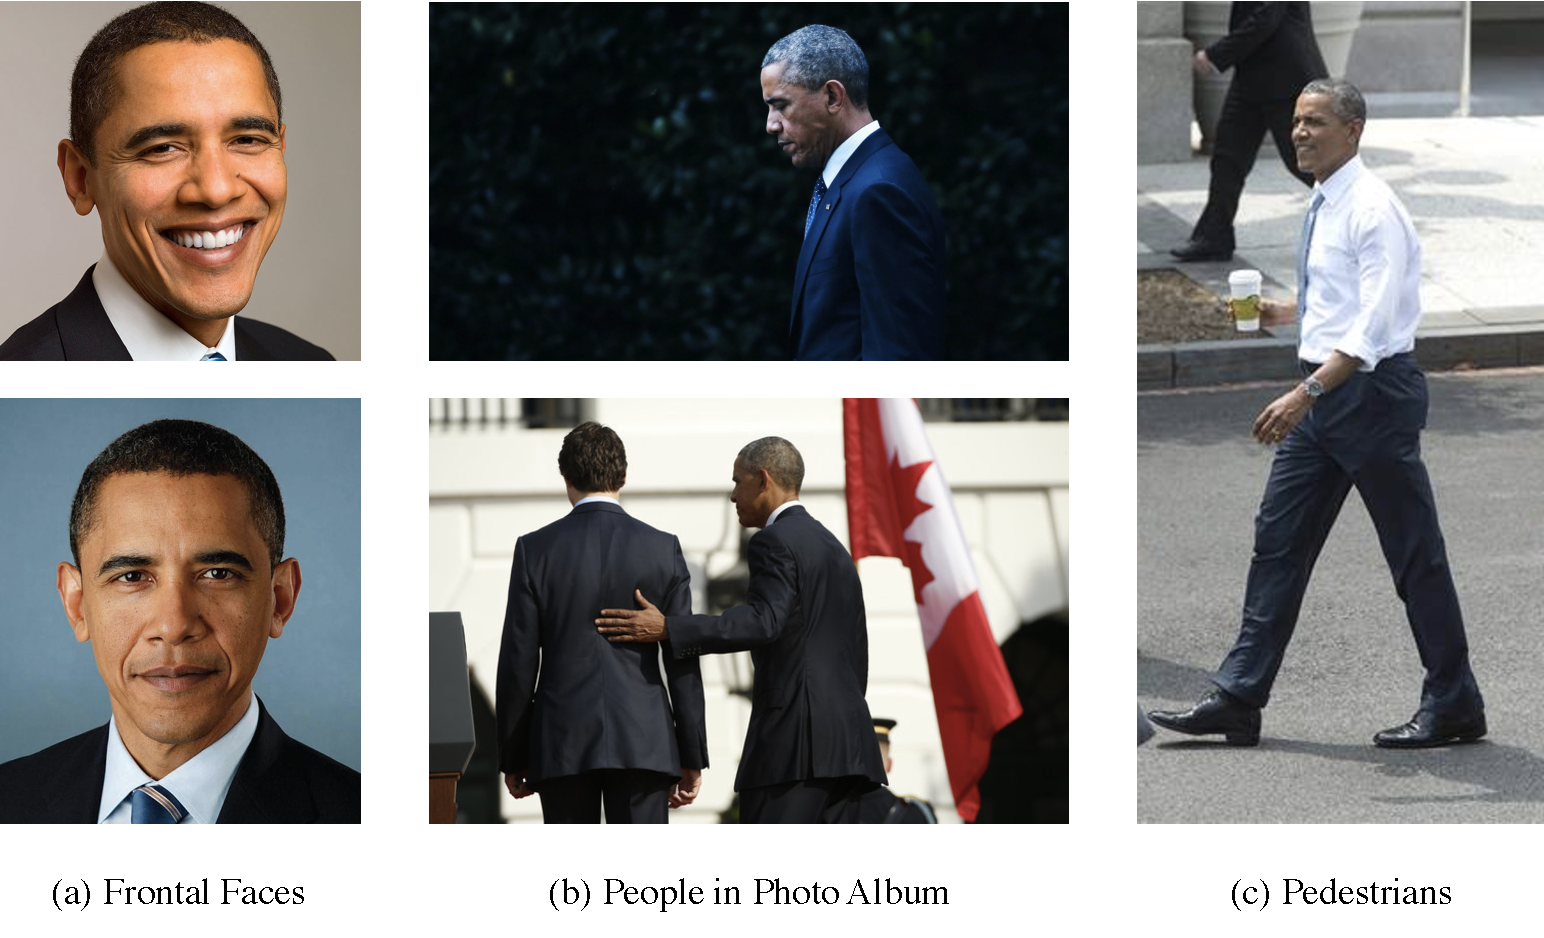
\includegraphics[width=1.0\linewidth]{figures/human-id.pdf}
\caption{Human identification with different types of input photos}
\label{fig:human-id-problems}
\end{center}
\end{figure}

Facial images are the easiest case among the three, as human faces are more rigid-like. Slight deformation only appears when the person has expressions. Thus computers can easily align different facial images and compare among them, which is well studied in~\cite{sun2014deep1,sun2014deep2,taigman2014deepface,parkhi2015deep}. However, in many cases human faces cannot be clearly captured, for example, there are many people profiles in our daily photo albums. It is much harder and requires utilizing multiple cues, including facial profile, hair styles, body shapes, and clothes to recognize a person~\cite{zhang2015beyond}.

Apart from these two types of human photos captured by normal digital cameras, surveillance cameras capture another type of people --- pedestrians. Due to the low resolution image with various weather and lighting conditions, as well as various human poses, recognizing pedestrians is very challenging. Researchers have named this problem setting \emph{Person Re-Identification (re-ID)}~\cite{zajdel2005keeping}. In this dissertation we also mainly focus on this setting.

\subsection{Evaluation Metrics} % (fold)
\label{sub:human-id-eval-metrics}
Despite the difference of image types, all these problem settings can be abstracted as follows. Given a photo of the person of interest, which is often called the \emph{query} or \emph{probe}, and a collection of images, which is called the \emph{gallery}, computers are required to rank the gallery images according to their similarity with the query photo.

\emph{Cumulative Matching Characteristics (CMC)} curves are the most popular evaluation metrics for such problem settings. Consider a simple single-gallery-shot setting, where each gallery identity has only one instance. For each query, an algorithm should rank all the gallery samples according to their distances to the query from small to large, and the CMC top-k accuracy is
\begin{equation}
  \mathrm{cmc}_k = \begin{cases}
    1 & \text{if the query identity is contained in the top-$k$ ranked gallery samples,} \\
    0 & \text{otherwise},
  \end{cases}
\end{equation}
which is a shifted step function. The final CMC curve is computed by averaging the shifted step functions over all the queries.

While the single-gallery-shot CMC is well defined, it does not have a common agreement when it comes to the multi-gallery-shot setting, where each gallery identity could have multiple instances. Authors of different datasets have defined different criterion. For example, CUHK03~\cite{li2014deepreid} and Market-1501~\cite{zheng2015scalable} calculate the CMC curves and CMC top-k accuracy quite differently. To be specific,

\begin{itemize}
  \item CUHK03: Query and gallery sets are from different camera views. For each query, they randomly sample one instance for each gallery identity, and compute a CMC curve in the single-gallery-shot setting. The random sampling is repeated for multiple times and the expected CMC curve is reported.
  \item Market-1501: Query and gallery sets could have same camera views, but for each individual query identity, his/her gallery samples from the same camera are excluded. They do not randomly sample only one instance for each gallery identity. This means the query will always match the ``easiest'' positive sample in the gallery while does not care other harder positive samples when computing CMC.
\end{itemize}
% subsection human-id-eval-metrics (end)

\subsection{Recent Advances} % (fold)
\label{sub:human-id-recent-adv}
Apart from the classical settings introduced above, researchers have recently extended the human identification problem from various aspects. For example, traditional person re-identification requires both query and gallery images to be manually cropped, while~\cite{xu2014person,xiaoli2017joint,zheng2017person} relaxed such constraints and considered detection with re-ID. Zheng \etal~\cite{zheng2016mars} explored person re-identification from videos rather than static images. Sometimes people do not have photo for the query person, for example, a criminal is only seen by a witness, in such case we can only rely on the testimony. Therefore, Li \etal~\cite{li2017person} proposed to replace the query image with text descriptions to search a person among gallery photos, which enriches the application scenarios of human identification.
% subsection human-id-recent-adv (end)
% section human-id-prob-settings (end)

\section{Technical Roadmap} % (fold)
\label{sec:human-id-tech-roadmap}
After introducing the problem settings for human identification, this section develops a technical roadmap for solving the problem, which reviews some existing approaches and enlightens future research.

Human identification should be addressed from three levels. At first, we only consider the information from a single image, and try to learn good features to represent the person's identity. Secondly, given two feature maps from a pair of images, we should develop methods to compare these two feature maps, and predict whether they belong to the same identity. At last, we could explore the structure of the whole gallery set, determining how the representations should be constructed for this set, and rank the gallery samples according to the query sample. We elaborate on these three aspects in Section~\ref{sub:human-id-feat-learn},~\ref{sub:human-id-feat-comp}, and~\ref{sub:human-id-structure-set}.

By interlacing human identification with other research fields we could advance the problem beyond the traditional image-based setting. For example, we may use natural language descriptions for querying a person instead of using the photo. Moreover, we could synthesize training data by exploiting generative models and rendering 3D models, which leverages the need of constructing large-scale supervised datasets. We introduce some recent advances towards these directions in Section~\ref{sub:human-id-data-modalities} and~\ref{sub:human-id-generative-models}.

\subsection{Identity Feature Learning} % (fold)
\label{sub:human-id-feat-learn}
The first fundamental question is how to learn discriminative feature representations for a single person image. Given an input image $x$, the objective is to learn a feature vector $f(x)$ such that the distance between the same identity $||f(x)-f(x^+)||_2$ (where $x$ and $x^+$ are images of the same identity) is small enough, while the distance among different people $||f(x)-f(x^-)||_2$ (where $x$ and $x^-$ are images of different people) is large enough.

Researchers have proposed various loss functions to learn such features. For example, Sun \etal~\cite{sun2014deep1,sun2014deep2} proposed to train the neural network to classify the identities with softmax cross entropy loss introduced in Section~\ref{sec:dl-loss}. Although it is indeed a surrogate loss function for feature learning, it works reasonably well in practice. Later on triplet loss is proposed~\cite{taigman2014deepface} that learns the features directly for ranking rather than classification. And Parkhi \etal~\cite{parkhi2015deep} combined both loss functions together in a multi-staged training process.

A disadvantage of triplet loss is that it can only compare one pair of samples at each time, which is inefficient and highly relies on good sampling strategies. Therefore, in Section~\ref{sec:ps-oim-loss} we proposed a novel loss function dubbed \emph{Online Instance Matching (OIM)} that compares the features among all identities at once. OIM loss absorbs the advantages from softmax and triplet loss but leaves their disadvantages behind. Several other recent work~\cite{wen2016discriminative,titsias2016one,snell2017prototypical} also explored similar ideas.
% subsection human-id-feat-learn (end)

\subsection{Feature Comparison} % (fold)
\label{sub:human-id-feat-comp}
After getting discriminative feature representations for each single image, the next question is how to compare a pair of image features. Prior to deep learning, many research focused on metric learning~\cite{davis2007information,weinberger2005distance,mcfee2010metric,koestinger2012large,liao2015person,zhang2016learning}, which learns a distance function $d(f(x_1), f(x_2))$ that replaces the conventional L2-distance. However when deep learning emerges, learning simple linear metrics can be casted to learning underlying features, which makes metric learning less significant.

Comparing a pair of deep learning feature maps is nontrivial, since the feature maps contain spatial information and the two feature maps are usually not well aligned, for example, the region of frontal face in one image could be just background in the other image. Li \etal~\cite{li2014deepreid} proposed a siamese deep learning architecture that computes the correlation between the strips on two feature maps, and estimates the similarity according to the correlation. Ahmed \etal~\cite{ahmed2015improved} further changed the correlation from strips to local rectangle regions, which significantly improved the performance. This feature maps matching problem is also closely related to the pixel correspondence problem for \emph{optical flow} estimation~\cite{weinzaepfel2013deepflow,revaud2016deepmatching}. One may get inspired from these work to design better architectures for capturing geometric transformations.
% subsection human-id-feat-comp (end)

\subsection{Structure of Feature Set} % (fold)
\label{sub:human-id-structure-set}
The last question is how to rank a set of gallery images according to the query. Answering this question requires modeling the structure of the gallery feature set. For example, by observing many gallery photos one can understand what the \emph{salient} features are for distinguishing different people~\cite{zhao2013unsupervised,zhao2017person}. Several other work focused on the ranking algorithm itself. Zhong \etal~\cite{zhong2017re} proposed a re-ranking algorithm by exploiting the prior knowledge that each identity has at least two instances in gallery set. Liu \etal~\cite{liu2013pop} designed an algorithm cooperate with human labelers to refine a initial ranking result.
% subsection human-id-structure-set (end)

\subsection{Data Modalities} % (fold)
\label{sub:human-id-data-modalities}
\begin{figure}[t]
\begin{center}
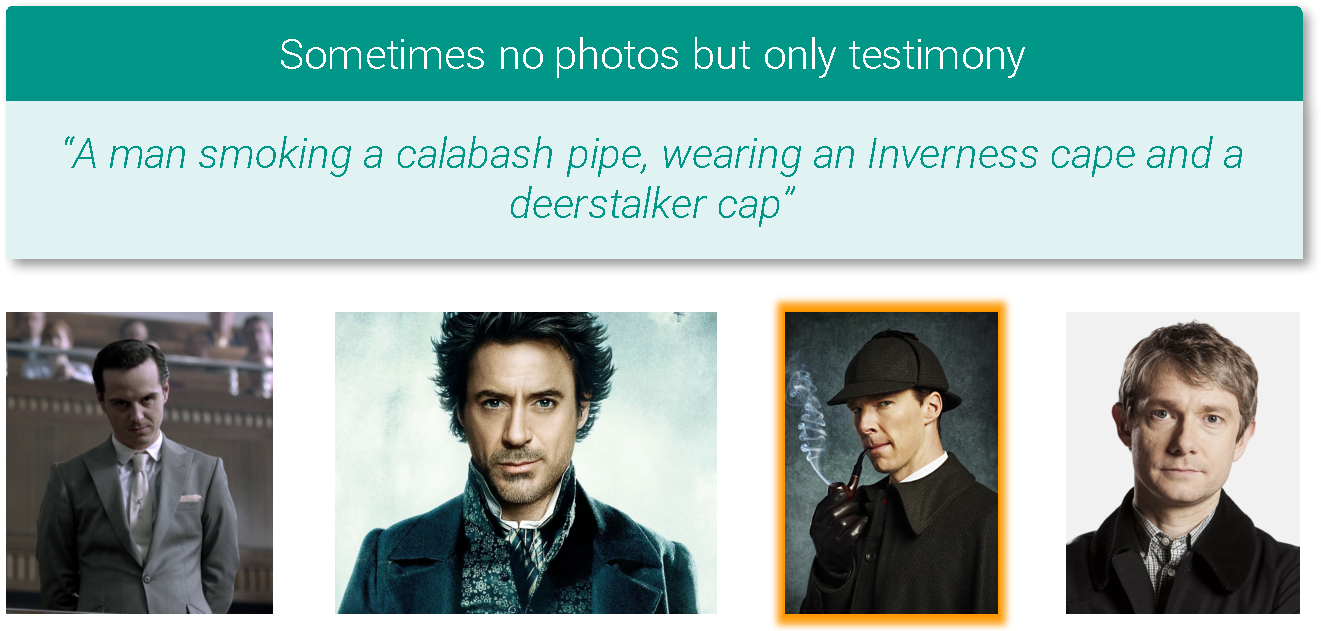
\includegraphics[width=1.0\linewidth]{figures/text-based-reid.pdf}
\caption{Human identification with natural language descriptions as query}
\label{fig:human-id-text-based-reid}
\end{center}
\end{figure}
In some real-world scenarios, we do not have photos for the query person, for example when catching a criminal, the police sometimes only have testimony from a witness, as demonstrated in Figure~\ref{fig:human-id-text-based-reid}. Studying different data modalities for human identification thus becomes very important for pushing it towards real applications. Li \etal~\cite{li2017person} introduced the person search problem with natural language description. They proposed a CNN-RNN architecture with attention mechanisms to solve the problem, and collected a dataset to validate their approach. It was further improved in~\cite{li2017identity} by exploiting the identity information to help feature learning.

The relationship between image modality and language modality has been actively studied in recent years from different aspects, including image captioning~\cite{karpathy2015deep,xu2015show,vinyals2015show,johnson2016densecap}, visual question answering (VQA)~\cite{antol2015vqa,ren2015exploring,malinowski2015ask,johnson2016clevr}, and text-based image retrieval~\cite{reed2016learning}. For human-identification, one intriguing property of using language modality is that it enriches the information we have. Traditionally, we only know whether each pair of people matches or not. With natural language descriptions, we can further know why they match and what the evidences are. These additional information could make the learned deep neural networks more discriminative and generalize better.
% subsection human-id-data-modalities (end)

\subsection{Generative Models and Rendering 3D Models} % (fold)
\label{sub:human-id-generative-models}
Learning well-performed deep neural networks currently requires large-scale supervised datasets, but collecting the data could be tedious and time consuming. To cope with this problem, recent work~\cite{richter2016playing,chen2017photographic} exploited computer graphics technologies that render 3D models to high-quality life-like 2D images. They showed that combining small amount of real data and numerous synthetic data could significantly improve the performance of deep neural networks for scene parsing.

One problem of using synthetic images is that when they are too different from real images, it could be meaningless to learn deep neural networks with them. To reduce the gap of the discrepancy between synthetic data and real data, Shrivastava \etal~\cite{shrivastava2017learning} exploit the \emph{Generative Adversarial Networks (GANs)} to transfer the synthetic images to real images. In the person re-identification literature, Zheng \etal~\cite{zheng2017unlabeled} use GAN to directly generate the person images, which serve as training data for training deep neural networks.
% subsection human-id-generative-models (end)

% section human-id-tech-roadmap (end)